\subsection{Automatically generating new questions}
One of the main problems with the application is generating entity model instances used for generating questions. To make one scenario with assessment, diagnosis, management and follow-up, we need at least two instances of the entity graph. One to show the status of the patient before the treatment, and one after the treatment. As the treatment needs to be evaluated and the clinician needs to act accordingly. One single entity model can be several hundreds of lines written in JSON, as there are quite many vertices and edges to describe, as well as the complexity of the model. This is tedious work, both because of the complexity, the amount of code lines, but the author also needs to put a great emphasize on writing the code correctly. The latter can be solved with an authoring tool.

As so much effort has to be put in typing these instances of entity graphs, a better way would be to make functionality to automatically generate new instances. We already have made templates with tags to vertices in the entity graph. By generating a lot of new entity instances, one template can be reused to make just as many questions. By looking at the paediatric possible asthma guideline \parencite{RepublicofKeny2016}, we see that there are described twelve symptoms we can combine in every way we like. Some of the symptoms also have more possibilities than just true/false. They have numerical ranges like pulse rate, breaths per minute and oxygen saturation. So in fact, we can generate a quite large amount of graph instances and equally as many questions per template.

The method we suggest for automatically generating such graph instances, is by introducing constraint checks in DPF. These constraint checks will be code which ensures that the vertices of the graph follows some predefined rules. For example, we know that the graph stores a boolean measurement value for wheeze. A constraint check will ensure that the value we generate for wheeze will be either true or false. For conciousness we have the enumeration values A, V, P and U. And we have value ranges, such as oxygen saturation and pulse rate. To get reasonable  constraints, a domain expert is needed to define the upper and lower limits a constraint should allow. For example a pulse rate for an old man shouldn't be set to 200 beats per minute, as his maximum pulse rate would be much lower than that.

However, some vertices are dependent on other vertices. For the paediatric guideline of possible asthma \parencite{RepublicofKeny2016}, wheeze will always have to be present to set an asthma diagnosis. For children less than 12 months, either or both of cough and difficulty breathing needs to be present in addition to wheeze. For the asthma to be severe, there are at least one additional symptom which needs to be present.

When the student will be asked for medication dosages, we know that some drugs may have standard measurements. For example, a medication we want to administer to patient, is 2.5mg per tablet. Then the dosage administered to the patient will be something which can be divided by 2.5. Here the dosages can be 2.5mg, 5mg, 7.5mg and so on.

Some of these constraints can be reused between guidelines. The same medication can be used for different diseases, as well as a person's maximum pulse rate probably will be the same whether he he has asthma or pneumonia. The AVPU-scale is a standard for measuring consciousness. However it can be tedious to get full constraint coverage, and when the guideline gets updated, we also need to update the constraints. In cases of not full constraint coverage, the entity instance graphs need to be validated by a domain expert, to see which of the generated instance graphs which can be used or not.  Even though this method relies on a domain expert, it will save us from a ton of work. Instead of carefully write hundreds of JSON formatted lines for each graph instance, we can simply approve or disapprove the graph instances which are valid or invalid. The constraints will also greatly reduce the noise the domain expert needs to go through. 



%\begin{figure}[h!]
%	\caption {The red and green graph instances at the bottom are picked from a repository. We randomly pick vertices from each entity instance to make the new entity instance at the bottom. Red vertices indicate that they come from the red entity graph instance. The green vertices that they come from the green entity graph instance.}
%	\label{fig:GeneratedEntityInstances}
%	\includegraphics[scale=0.35]{GeneratedEntityInstances}
%\end{figure}

When we have built up a repository of entity graph instances, we can use this repository to generate distractions for quiz elements. Randomly choose distractions from other entity graph instances, which corresponds to the answer key tag given by the template. A small penalty can be set on distractions from the asthma guideline. Medium penalties for distractions from respiratory diseases. A bit larger penalties for distractions from completely unrelated guidelines. Then we have automated the quiz scores as well!

\subsection{Dissemination of guidelines}
At one point we want to have a game, where the student can choose between many different quizzes where he will be tested in different guidelines for different medical conditions. These guidelines has to be managed from somewhere. New questions arrives: should all the guidelines be packed with the game application itself? Or should the student install quizzes for just the guidelines he is interested in? When there is a change in a clinical practice guideline. How do we make sure that the clinician trains with the most recent quiz version?

Our suggestion is that the game comes with a predefined set of quizzes for the most used guidelines. Then the clinician can install quizzes or categories of quizzes which he is the most interested in. The application automatically checks for new versions when the application starts. The quizzes needs to have a version tag, such that version checking can be possible.

\subsection{Scalability}
How do we train, 10, 100, 1000 clinicians? Our solution so far is that the clinicians are responsible and in charge of their own training. Another scenario can be a teacher or a course leader having many students. The application can track the student's knowledge level in quizzes of interest and the progression of the student. The student can submit their data to a central server, where individual and collective skill and progress of the students can be visualized through chart and statistics for the teacher. In this way he can better target students which is in need for individual help, or subjects where the class is weak and should be addressed by the teacher.

\subsection{Multimedia as part of the quiz questions}
In the evaluation of the application, we saw that some of the clinicians wanted pictures and sound as part of the questions. Pictures, sound and video is far more similar the situations the clinicians meet at the hospital. Where they need to look, listen and observe the patient, rather than having the examination results handed to them in a text format. 

One way to integrate multimedia into the questions, is by meta tagging the important observations done in the videos, pictures and sound. Then we can build an instance of a specific entity model for that video, picture or a sound.

For example: a sound clip of a wheezing sound would have a graph is modelled in figure \ref{fig:WheezeSound}. By subtracting this graph from the one used for textual questions, we don't get wheeze as a part of the textual question. The student needs to listen and analysing the sound to understand that the patient is wheezing.

\begin{figure}[h!]
	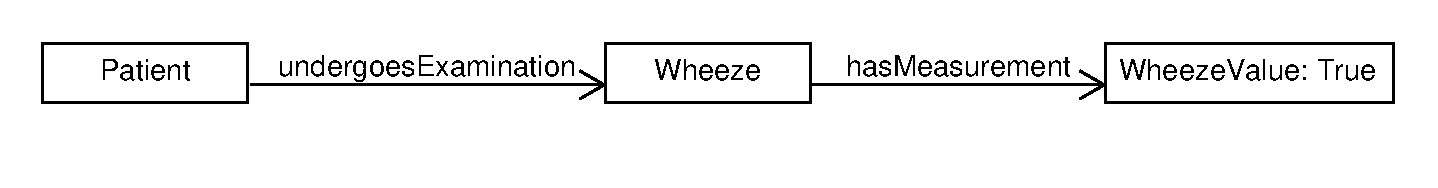
\includegraphics[scale=0.5]{WheezeSound}
	\caption {An entity instance of the wheezing sound}
	\label{fig:WheezeSound}
\end{figure}

We can use this method in combination with other types of pictures. A patient laying in the bed with a facial mask, tells that this is a patient which has been treated with oxygen. As the patient is not alert, the patient is probably still having severe asthma. This is information which can be removed from the textual question when we have a graph which tells that this can be seen in the picture.

From a picture it is also easy to see if the patient is either a child, an adult and where he is located. A picture of a child playing with his toys could be mild or moderate asthma as he is alert. A patient which doesn't respond to the questions from the doctor, could be severe asthma as he is showing an inability to talk because of the breathing difficulties.

